\section{Neural Networks}\label{sec:neural-networks}
Without further ado, we will discuss what neural networks are and how they are composed.
We describe what a layer is and what types there are.
For what do we need optimizers and activation functions and what types are there.
Neural Networks are useful in a multitude of fields like classification, regression, transcription, or machine translation. \cite{goodfellow_deep_2016}
Neuronal networks are composed of layers, which are composed of neurons.
The neuron is the computational component in a deep neural network.\\
A neuron transforms a vector of inputs $\mathbf{x}$ to the output $y$, $\mathbb{R}^n \to \mathbb{R}$
by using a vector of weights $\mathbf{w}$, a bias $b$ and an activation function $f$ \ref{eq: NeuralFunction}.
\begin{equation}
    y = f\left( \sum^n_{i=1} w_i\cdot x_i + b\right)
    \label{eq: NeuralFunction}
\end{equation}
For Example, in the machine learning software library TensorFlow, which is based on Keras, uses by default Glorot uniform initializer\cite{noauthor_tfkeraslayersdense_nodate,glorot_understanding_2010},
also called Xavier uniform initializer for the weights and initializes the bias with zeros.\\
Another important component, are the activation functions, one of the most common ones is the sigmoid function, which is today mostly used in output layers.
The rectified linear unit, short ReLU \ref{eq: relu} which was first used 1975 by Fukushima\cite{fukushima_cognitron_1975} and shown in 2011 by Glorot et al. \cite{glorot_deep_2011}
that it enables a better training for a neural network compared to the till then common sigmoid function.
\begin{equation}
    f(x) =
    \begin{cases}
        x& x > 0\\
        0& x <= 0
    \end{cases}
    \label{eq: relu}
\end{equation}
Another even more promising activation function is the Gaussian Error Linear Unit, short GELU \ref{eq: relu} which was proposed by Hendrycks and Gimpel in 2016\cite{hendrycks_gaussian_2016} is used by natural language processing models like BERT\cite{devlin_bert_2019}.
It does not just set all negative values to zero like ReLU but weights them.
The differences can be seen in the figure. \ref{fig: activation function}
\begin{equation}
    f(x) = 0.5x\left ( 1+\tanh\left [ \sqrt{\frac{2}{\pi}}\left ( x+0.044715x^3 \right ) \right ] \right )
    \label{eq: gelu}
\end{equation}
\begin{figure}
    \centering
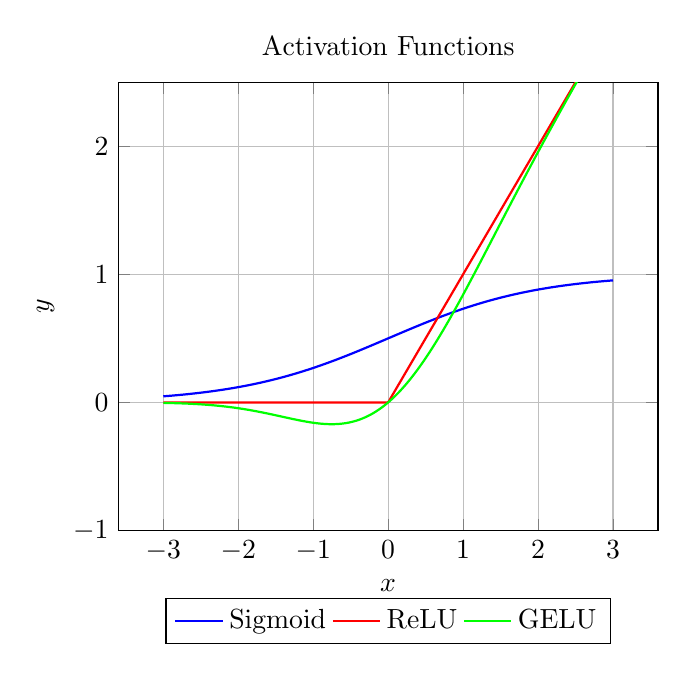
\begin{tikzpicture}
    \begin{axis}[
        title={Activation Functions},
        xlabel={$x$},
        ylabel={$y$},
        domain=-3:3, % Adjust the domain for a narrower x-axis range
        ymin=-1, % Set y-minimum
        ymax=2.5, % Set y-maximum
        samples=400, % Increase the number of samples for a smoother curve
        grid=both,
        legend style={at={(0.5,-0.15)}, anchor=north,legend columns=3},
      ]
      \addplot[blue, thick] {1/(1 + exp(-x))};
      \addplot[red, thick] {max(0, x)};
      \addplot[green, thick] {0.5*x*(1 + tanh(sqrt(2/pi)*(x + 0.044715*x^3)))};
      \legend{Sigmoid, ReLU, GELU}
    \end{axis}
  \end{tikzpicture}
  \caption{Activation Functions}
  \label{fig: activation function}
\end{figure}
The neurons are then combined into layers, in a Deep Neural Network (DNN) we have three types of Layers:
Input layers, output layers and the hidden layers.
In general are there is only one input and one output layer \ref{fig: neural network}, but there is a plurality of hidden layers.
The input layer, is pretty straightforward, it processes the input for the hidden layers, for example, it converts a 2-dimensional picture to a 1-dimensonal array,
which can then be processed by the subsequent layers.
The hidden layer does most of the heavy lifting, it performs most of the computational work of a DNN, it works based on the formula from above.
The output layer, takes the output of the last hidden layer, transforms it so that we get a meaningful output.
For a regression or binary classification, we have mostly just one neuron, but for a multi-class classification the number of neurons corresponds with the number of classes that shall be classified.
The output layer also works after the same principle of the formula above, but not a “normal” activation function is used.
Either a no activation function is used or a linear activation function is used for a regression or the softmax \ref{eq: softmax} function for a classification model.
\begin{equation}
    f(x_i) = \frac{e^{x_i}}{\sum^n_{j=1}e^{x_j}}
    \label{eq: softmax}
\end{equation}
\begin{figure}
  \centering
  % Input layer neurons'number
  \newcommand{\inputnum}{5}

  % Hidden layer neurons'number
  \newcommand{\hiddennuma}{6}
  \newcommand{\hiddennumb}{8}
  \newcommand{\hiddennumc}{5}

  % Output layer neurons'number
  \newcommand{\outputnum}{4}

  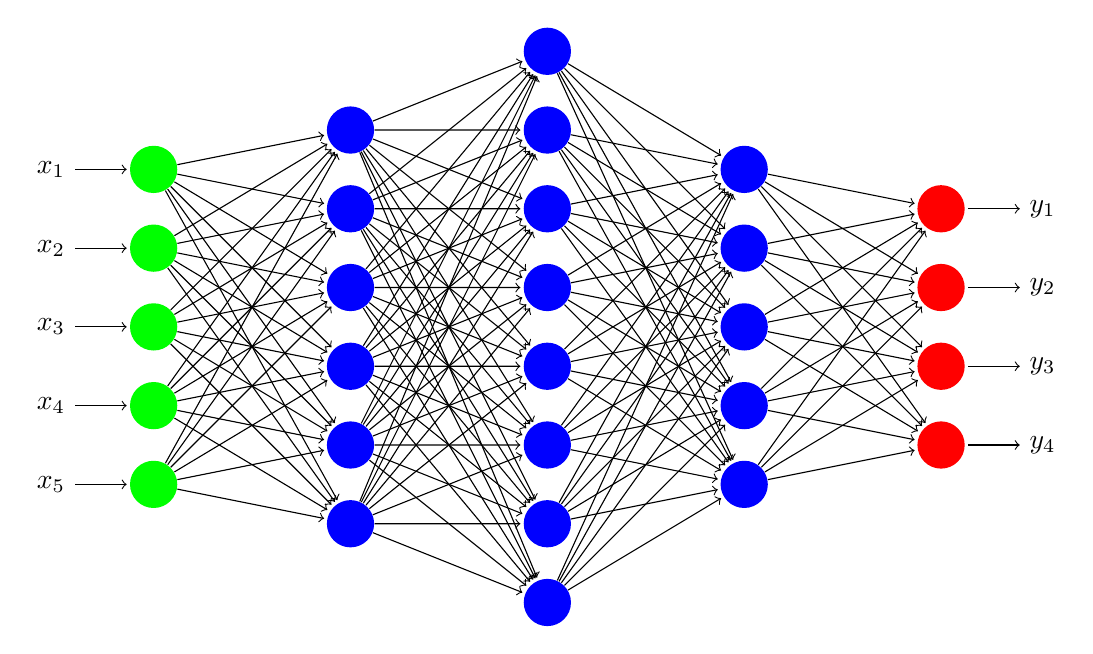
\begin{tikzpicture}

    % Input Layer
    \foreach \i in {1,...,\inputnum}
    {
	  \node[circle,
		minimum size = 6mm,
		fill=green] (Input-\i) at (0,-\i) {};
    }

    % Hidden Layer
    \foreach \i in {1,...,\hiddennuma}
    {
      \node[circle,
		minimum size = 6mm,
		fill=blue,
		yshift=(\hiddennuma-\inputnum)*5 mm
	  ] (HiddenA-\i) at (2.5,-\i) {};
    }

    \foreach \i in {1,...,\hiddennumb}
    {
	  \node[circle,
		minimum size = 6mm,
		fill=blue,
		yshift=(\hiddennumb-\inputnum)*5 mm
	  ] (HiddenB-\i) at (5,-\i) {};
    }

    \foreach \i in {1,...,\hiddennumc}
    {
	  \node[circle,
		minimum size = 6mm,
		fill=blue,
		yshift=(\hiddennumc-\inputnum)*5 mm
	  ] (HiddenC-\i) at (7.5,-\i) {};
    }

    % Output Layer
    \foreach \i in {1,...,\outputnum}
    {
	  \node[circle,
		minimum size = 6mm,
		fill=red,
		yshift=(\outputnum-\inputnum)*5 mm
	  ] (Output-\i) at (10,-\i) {};
    }

    % Connect neurons In-Hidden
    \foreach \i in {1,...,\inputnum}
    {
	  \foreach \j in {1,...,\hiddennuma}
	  {
		\draw[->, shorten >=1pt] (Input-\i) -- (HiddenA-\j);
	  }
    }

    % Connect neurons Hidden
    \foreach \i in {1,...,\hiddennuma}
    {
	  \foreach \j in {1,...,\hiddennumb}
	    {
		  \draw[->, shorten >=1pt] (HiddenA-\i) -- (HiddenB-\j);
	  }
    }

    \foreach \i in {1,...,\hiddennumb}
    {
	  \foreach \j in {1,...,\hiddennumc}
	    {
		  \draw[->, shorten >=1pt] (HiddenB-\i) -- (HiddenC-\j);
	  }
    }

    % Connect neurons Hidden-Out
    \foreach \i in {1,...,\hiddennumc}
    {
	  \foreach \j in {1,...,\outputnum}
	    {
		\draw[->, shorten >=1pt] (HiddenC-\i) -- (Output-\j);
	}
  }

  % Inputs
  \foreach \i in {1,...,\inputnum}
    {
	  \draw[<-, shorten <=1pt] (Input-\i) -- ++(-1,0)
		node[left]{$x_{\i}$};
    }

  % Outputs
  \foreach \i in {1,...,\outputnum}
    {
	  \draw[->, shorten <=1pt] (Output-\i) -- ++(1,0)
		node[right]{$y_{\i}$};
    }

  \end{tikzpicture}
  \caption{Neural Network}
  \label{fig: neural network}
  \fcolorbox{black}{green}{\rule{0pt}{6pt}\rule{6pt}{0pt}}\quad Input Layer \quad
  \fcolorbox{black}{blue}{\rule{0pt}{6pt}\rule{6pt}{0pt}}\quad Hidden Layer \quad
  \fcolorbox{black}{red}{\rule{0pt}{6pt}\rule{6pt}{0pt}}\quad Output Layer
\end{figure}
But, how are deep neural networks trained? \cite{lecun_deep_2015}
The first step is forward propagation, the training data is fed in to the network and flows through the layers, where each neuron performs it operation. \ref{eq: NeuralFunction}
Afterwards the backpropagation or backpropagation of error is performed. \cite{rumelhart_learning_1986}
Then the output is compared to the desired outcome of the training data, hence, if the predicted outcome of the network matches the actual outcome.
If it doesn't match, it calculates how far off the prediction is.
Subsequently, the process of backpropagation is initiated, wherein the error determined in the preceding step is propagated through the network.
Then the weights are updated, often a process called stochastic gradient descent (SGD) is used.
In SGD, a few examples of the input are used, to compute the output and the error, then the average gradient for the examples is used, to adjust the weights.
Then this process is repeated until we are gone through the whole training set, which is called an epoch.
\subsection{Core Layers in Neural Networks}\label{subsec:core-layers-in-neural-networks}
\subsubsection{Dense Layers}
Dense Layers are the backbone of neural networks.
They do most of the computational work of a neural network.
It's characterized by its fully connected architecture, like seen in the figure \ref{fig: neural network}, meaning every node of the layer is connected to every node of the predecessor layer and every node of the successor layer.
Dense layers are pivotal in learning intricate patterns from data, their versatility allows them to be stacked where each layer captures different levels of data abstraction.
They work internally, like in the function above \ref{eq: NeuralFunction}.
\subsubsection{Convolutional Layer}
Convolutional layers, are used in image processing\cite{lecun_backpropagation_1989,szegedy_going_2014,krizhevsky_imagenet_2012}, unlike dense layers that try to analyse an image as a whole, but uses the concept of convolution to get a set of smaller pictures which depict isolated features of a picture.
A convolution describes how a function f is modified by a function g, for example in the discrete case: \ref{eq: convolution}.
\begin{equation}
(f \ast g)[n] = sum_{m=-\inf}^{\inf}f[m]\cdot g[n - m]
    \label{eq: convolution}]
\end{equation}
But how does this correspond to neural networks and image processing, foremost, we have not 1Dimensional data, but 2Dimensional pictures. \ref{eq: 2Dconvolution} \ref{fig: convolution matrix}
\begin{equation}
(f \ast g)[x,y] = \sum^{\inf}_{m=-\inf} \sum^{\inf}_{n=-\inf} f[m,n]\cdot g[x-m,y-n]
    \label{eq: 2Dconvolution}
\end{equation}
\input{figures/convolution.tikz}
For this, the singular weights are replaced by matrices of weights, so-called kernels or filters.
The output of the convolutional layer, are so-called feature maps, each of these contains the result of applying one filter to the input data.
These capture different aspects, like edges or textures.
There are two other variables in a convolutional layer, apart from the number of the number and size of filters and the activation function.
They are the stride and the padding, the stride describes how many steps the filter moves between successive convolutions.
The larger stride, the smaller the resulting filter map, and vice versa.
Of course, a larger stride results in less detail in a map.
Padding is an optional parameter which aids in maintaining information on the edge of an input and helps to keep the scale of a picture.
\subsubsection{Pooling Layer}
\begin{figure}[h]
\centering
\begin{tikzpicture}[
    2d-arr/.style={matrix of nodes, row sep=-\pgflinewidth, column sep=-\pgflinewidth, nodes={draw}}
  ]

  \matrix (mtr) [2d-arr] {
  |[fill=red!30]| 3 & |[fill=red!30]| 4 & |[fill=blue!30]| 6 & |[fill=blue!30]| 7\\
  |[fill=red!30]| 4 & |[fill=red!30]| 1 & |[fill=blue!30]| 2 & |[fill=blue!30]| 9\\
  |[fill=green!30]| 6 & |[fill=green!30]| 6 & |[fill=yellow!30]| 2 & |[fill=yellow!30]| 3\\
  |[fill=green!30]| 7 & |[fill=green!30]| 1 & |[fill=yellow!30]| 6 & |[fill=yellow!30]| 5\\
  };

  \node[right=0.2em of mtr] (str) {$\Longrightarrow$};

  \matrix (K) [2d-arr, right=0.2em of str] {
    |[fill=red!30]| 4 & |[fill=blue!30]| 9 \\
    |[fill=green!30]| 7 & |[fill=yellow!30]| 6 \\
  };

\end{tikzpicture}
\begin{tikzpicture}[
    2d-arr/.style={matrix of nodes, row sep=-\pgflinewidth, column sep=-\pgflinewidth, nodes={draw}}
  ]

  \matrix (mtr) [2d-arr] {
  |[fill=red!30]| 3 & |[fill=red!30]| 4 & |[fill=blue!30]| 6 & |[fill=blue!30]| 7\\
  |[fill=red!30]| 4 & |[fill=red!30]| 1 & |[fill=blue!30]| 2 & |[fill=blue!30]| 9\\
  |[fill=green!30]| 6 & |[fill=green!30]| 6 & |[fill=yellow!30]| 2 & |[fill=yellow!30]| 3\\
  |[fill=green!30]| 7 & |[fill=green!30]| 1 & |[fill=yellow!30]| 6 & |[fill=yellow!30]| 5\\
  };

  \node[right=0.2em of mtr] (str) {$\Longrightarrow$};

  \matrix (K) [2d-arr, right=0.2em of str] {
    |[fill=gray!30]| 9\\
  };
\end{tikzpicture}
\caption{Max Pooling}
\label{fig: Max Pooling}
Left: Max Pooling, Filter: (2,2) Stride: 2 Right: Max Global Pooling
\end{figure}
\begin{figure}[h]
\centering
\begin{tikzpicture}[
    2d-arr/.style={matrix of nodes, row sep=-\pgflinewidth, column sep=-\pgflinewidth, nodes={draw}}
  ]

  \matrix (mtr) [2d-arr] {
  |[fill=red!30]| 3 & |[fill=red!30]| 4 & |[fill=blue!30]| 6 & |[fill=blue!30]| 7\\
  |[fill=red!30]| 4 & |[fill=red!30]| 1 & |[fill=blue!30]| 2 & |[fill=blue!30]| 9\\
  |[fill=green!30]| 6 & |[fill=green!30]| 6 & |[fill=yellow!30]| 2 & |[fill=yellow!30]| 3\\
  |[fill=green!30]| 7 & |[fill=green!30]| 1 & |[fill=yellow!30]| 6 & |[fill=yellow!30]| 5\\
  };

  \node[right=0.2em of mtr] (str) {$\Longrightarrow$};

  \matrix (K) [2d-arr, right=0.2em of str] {
    |[fill=red!30]| 1 & |[fill=blue!30]| 2 \\
    |[fill=green!30]| 1 & |[fill=yellow!30]| 2 \\
  };

\end{tikzpicture}
\begin{tikzpicture}[
    2d-arr/.style={matrix of nodes, row sep=-\pgflinewidth, column sep=-\pgflinewidth, nodes={draw}}
  ]

  \matrix (mtr) [2d-arr] {
  |[fill=red!30]| 3 & |[fill=red!30]| 4 & |[fill=blue!30]| 6 & |[fill=blue!30]| 7\\
  |[fill=red!30]| 4 & |[fill=red!30]| 1 & |[fill=blue!30]| 2 & |[fill=blue!30]| 9\\
  |[fill=green!30]| 6 & |[fill=green!30]| 6 & |[fill=yellow!30]| 2 & |[fill=yellow!30]| 3\\
  |[fill=green!30]| 7 & |[fill=green!30]| 1 & |[fill=yellow!30]| 6 & |[fill=yellow!30]| 5\\
  };
  
  \node[right=0.2em of mtr] (str) {$\Longrightarrow$};

  \matrix (K) [2d-arr, right=0.2em of str] {
    |[fill=gray!30]| 1\\
  };
\end{tikzpicture}
\caption{Min Pooling}
\label{fig: Min Pooling}
Left: Min Pooling, Filter: (2,2) Stride: 2 Right: Min Global Pooling
\end{figure}
\begin{figure}[h]
\centering
\begin{tikzpicture}[
    2d-arr/.style={matrix of nodes, row sep=-\pgflinewidth, column sep=-\pgflinewidth, nodes={draw}}
  ]

  \matrix (mtr) [2d-arr] {
  |[fill=red!30]| 3 & |[fill=red!30]| 4 & |[fill=blue!30]| 6 & |[fill=blue!30]| 7\\
  |[fill=red!30]| 4 & |[fill=red!30]| 1 & |[fill=blue!30]| 2 & |[fill=blue!30]| 9\\
  |[fill=green!30]| 6 & |[fill=green!30]| 6 & |[fill=yellow!30]| 2 & |[fill=yellow!30]| 3\\
  |[fill=green!30]| 7 & |[fill=green!30]| 1 & |[fill=yellow!30]| 6 & |[fill=yellow!30]| 5\\
  };

  \node[right=0.2em of mtr] (str) {$\Longrightarrow$};

  \matrix (K) [2d-arr, right=0.2em of str] {
    |[fill=red!30]| 3 & |[fill=blue!30]| 6 \\
    |[fill=green!30]| 5 & |[fill=yellow!30]| 4 \\
  };

\end{tikzpicture}
\begin{tikzpicture}[
    2d-arr/.style={matrix of nodes, row sep=-\pgflinewidth, column sep=-\pgflinewidth, nodes={draw}}
  ]

  \matrix (mtr) [2d-arr] {
  |[fill=red!30]| 3 & |[fill=red!30]| 4 & |[fill=blue!30]| 6 & |[fill=blue!30]| 7\\
  |[fill=red!30]| 4 & |[fill=red!30]| 1 & |[fill=blue!30]| 2 & |[fill=blue!30]| 9\\
  |[fill=green!30]| 6 & |[fill=green!30]| 6 & |[fill=yellow!30]| 2 & |[fill=yellow!30]| 3\\
  |[fill=green!30]| 7 & |[fill=green!30]| 1 & |[fill=yellow!30]| 6 & |[fill=yellow!30]| 5\\
  };

  \node[right=0.2em of mtr] (str) {$\Longrightarrow$};

  \matrix (K) [2d-arr, right=0.2em of str] {
    |[fill=gray!30]| 4.5\\
  };

\end{tikzpicture}
\caption{Average Pooling}
\label{fig: Average Pooling}
Left: Average Pooling, Filter: (2,2) Stride: 2 Right: Average Global Pooling
\end{figure}
\subsection{Optimization in Neural Networks}\label{subsec:optimization-in-neural-networks}
\section{Neural Network Testing}\label{sec:neural-network-testing}
\lipsum[21-25]
\section{Mutation-based Testing}\label{sec:mutation-based-testing}
\lipsum[26-30]
\section{Spectrum Analysis}\label{sec:spectrum-analysis}
\lipsum[31-35]
\section{DeepFault}\label{sec:deepfault}\cite{wong_dstar_2014}
\lipsum[36-40]